\subsection{Esercizio 15}
Eseguendo il codice \nameref{cod:15} si ottengono i seguenti risultati:

    
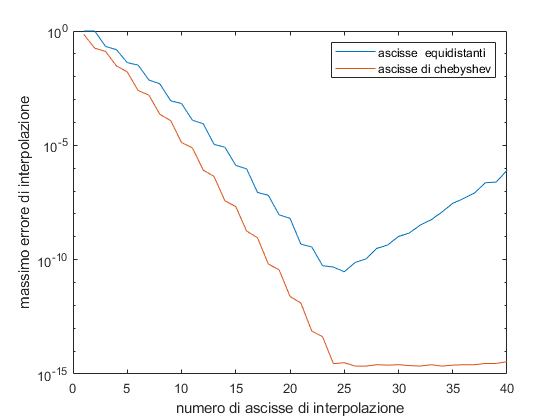
\includegraphics[scale=0.8]{capitolo4/interpol.png}

Si vede come, al crescere di n, torni a crescere anche l'errore quando si utilizzano le ascisse equidistanti, a differenza delle ascisse di chebyshev.